%\chapter*{ANNEXE}
%\pagenumbering{alph}
\renewcommand{\thesection}{\Alph{section}}
\pagenumbering{alph}

\setcounter{section}{0}

\begin{appendices}%\renewcommand{\thesection}{\Alph{section}}
\appendixheaderon

\section{Méthode de travail agile : SCRUM}
\label{ann:annexe1}
\subsection{Rôles}
\begin{enumerate}[parsep=0cm,itemsep=0cm]
\item \textbf{ Le \textit{«Product Owner»} ou \textit{«PO»} }: il porte la vision du produit à réaliser. Il travaille en collaboration directe avec l’équipe de développement et a notamment la charge de remplir le\textit{ «Product Backlog»} et de déterminer la priorité des \textit{«user stories»}\footnote{phrase simple, rédigée dans un langage courant, qui permet de décrire avec suffisamment de précision le contenu d’une fonctionnalité\\} à réaliser. 

\item \textbf{Le \textit{«Scrum Master»} ou \textit{«SM»}} : Il ne faut surtout pas le confondre avec un chef de projet. Il facilite le dialogue et le travail entre les différents intervenants, de façon à ce que l’équipe soit pleinement productive. 

\item \textbf{L’équipe de développement} : généralement composée de 4 à 6 personnes de plusieurs profils, elle est chargée de transformer les besoins exprimés par le \textit{«Product Owner»}  en fonctionnalités réelles, opérationnelles et utilisables. 
\end{enumerate}

\subsection{Réunions}
\begin{enumerate}[parsep=0cm,itemsep=0cm]
\item \textbf{Planification du \textit{Sprint}} (Sprint = itération) : au cours de cette réunion, l'équipe de développement sélectionne les éléments prioritaires du \textit{«Product Backlog»}\footnote{liste ordonnancée des exigences fonctionnelles et non fonctionnelles du projet} qu'elle pense pouvoir réaliser au cours du \textit{Sprint}.

\item \textbf{Revue de Sprint} : au cours de cette réunion qui a lieu à la fin du \textit{Sprint}, l'équipe de développement présente les fonctionnalités terminées au cours du \textit{Sprint} et recueille les feedbacks du \textit{«Product Owner»} et des utilisateurs finaux. C'est également le moment d'anticiper le périmètre des prochains \textit{Sprints} et d'ajuster au besoin la planification de \textit{release} (nombre de \textit{Sprints} restants).

\item \textbf{Rétrospective de \textit{Sprint}} : la rétrospective qui a généralement lieu après la revue de \textit{Sprint} est l'occasion de s'améliorer (productivité, qualité, efficacité, conditions de travail, etc) à la lueur du "vécu" sur le \textit{Sprint} écoulé (principe d'amélioration continue).

\item \textbf{Mêlée quotidienne}  : il s'agit d'une réunion de synchronisation de l'équipe de développement qui se fait debout en 15 minutes maximum au cours de laquelle chacun répond principalement à 3 questions : \textit{«Qu'est ce que j'ai terminé depuis la dernière mêlée ? Qu'est ce que j'aurai terminé d'ici la prochaine mêlée ? Quels obstacles me retardent ?»}.
\end{enumerate}

\subsection{Artefacts}
\begin{enumerate}[parsep=0cm,itemsep=0cm]
\item \textbf{Le \textit{Sprint}}: il s'agit d'une période pendant laquelle un travail spécifique doit être mené à bien avant de faire l'objet d'une révision.
\item \textbf{Le \textit{Product Backlog}}: il s'agit d'une liste hiérarchisée des exigences initiales du client concernant le produit à réaliser.
\item \textbf{Le \textit{Sprint Backlog}}: c'est le plan détaillé de la réalisation de l'objectif du \textit{Sprint}, défini lors de la réunion de planification du \textit{Sprint}.
\item \textbf{Le \textit{Task Board}} : outil central du \textit{Sprint} scrum, ce tableau de bord du projet permet de suivre en temps réel la progression de la réalisation des différentes tâches. Il pr\'esente les tâches à faire, les tâches en cours et les tâches terminées.
\item \textbf{Le \textit{Burndown Chart}} : il s’agit d’un graphique simple permettant de visualiser le degré d’avancement de chacune des tâches.
\end{enumerate}

\end{appendices}

\section{Compl\'ement sur les distances}
On retiendra essentiellement \cite{bensalem}:
\begin{itemize}[parsep=0cm,itemsep=0cm]
\item pour les mesures impliquant des chaînes de caractères on a les mesures lexicographiques (distances Levenshtein, distance Q-gram, distance de Jaro-Winkler) et les mesures phon\'etiques (Soundex, Double Metaphore, New York State Identification and Intelligence System, une combinaison des mesures phon\'etique et lexicographique);
\item pour les donn\'ees num\'eriques une transformation en chaînes de caractères peut \^etre appliqu\'ee;
\item pour les dates on peut effectuer un calcul de différence entre les jours, les mois et les années
\end{itemize} 


\section{Pr\'esentation des fichiers de configuration des jobs}
La validation des diff\'erentes attentes passe par l'\'ecriture des mesures y aff\'erentes. Le module Measure a besoin de deux fichiers pour configurer l'ex\'ecution du job Spark: \emph{env.json} et celui des mesures. Le fichier \emph{env.json} configure notamment trois grands points. On y retrouve les param\`etres pour l'ex\'ecution sur Spark aussi bien en cas de donn\'ees en \textit{batch} qu'en \textit{streaming}. Ensuite, la configuration pour la persistance des m\'etriques: affichage en console, sauvegarde sur \acrshort{hdfs} (\acrlong{hdfs}) ou sur Elasticsearch, ou encore une destination personnalis\'ee. Le dernier point concerne les points de contr\^ole pour les donn\'ees en \textit{streaming}. 
Le fichier destin\'e \`a la d\'efinition des mesures contient quant \`a lui principalement les param\`etres suivants:
\begin{description}[parsep=0cm,itemsep=0cm]
\item[name] : ce param\`etre permet de nommer le job qui sera ex\'ecut\'e; 
\item[process.type]: deux valeurs sont admises ici :  "BATCH" ou "STREAMING". Comme on peut le remarquer, cette variable est ajust\'ee en fonction du type de donn\'ees; 
\item[data.sources] : il s'agit d'une liste contenant les diff\'erentes sources de donn\'ees. On peut se connecter directement \`a plusieurs tables en m\^eme temps. La configuration de la source de donn\'ees requiert la d\'efinition du type de connexion (\acrshort{jdbc}, HIVE, AVRO, CUSTOM) et un paramétrage des acc\`es en fonction du type choisi; 

\item[evaluate.rule] : il s'agit d'un attribut contenant une liste de r\`egles \`a \'evaluer. Une r\`egle est d\'efinie en pr\'ecisant le langage utilis\'e (\textbf{dsl.type}). Deux types de langages sont support\'es par Griffin. On a  essentiellement \emph{spark-sql} et \emph{griffin-dsl}. Il faut \'egalement pr\'eciser la dimension de qualit\'e des donn\'ees (profiling, accuracy, completeness, uniqueness, timeliness) qui est \'evalu\'ee (\textbf{dq.type}), la r\`egle (\textbf{rules}) en elle-m\^eme ainsi que les modalit\'es de sorties (\textbf{out});
\item[sinks]: permet de lister les diff\'erentes sorties pour la persistance des m\'etriques.
\end{description}
\vspace{0.15cm}


%\vspace{0.5cm}

\section{Validation des \textit{tokens}}
Pour valider les tokens, nous avons t\'el\'echarg\'e et utilis\'e une base de donn\'ees test. Cette base mod\'elise l'activit\'e d'un a\'eroport. On y trouve huit (8) tables. \\
\begin{figure}[H]
 \caption{Mod\`ele des donn\'ees de test}  \label{fig:xray}
    \begin{center}
      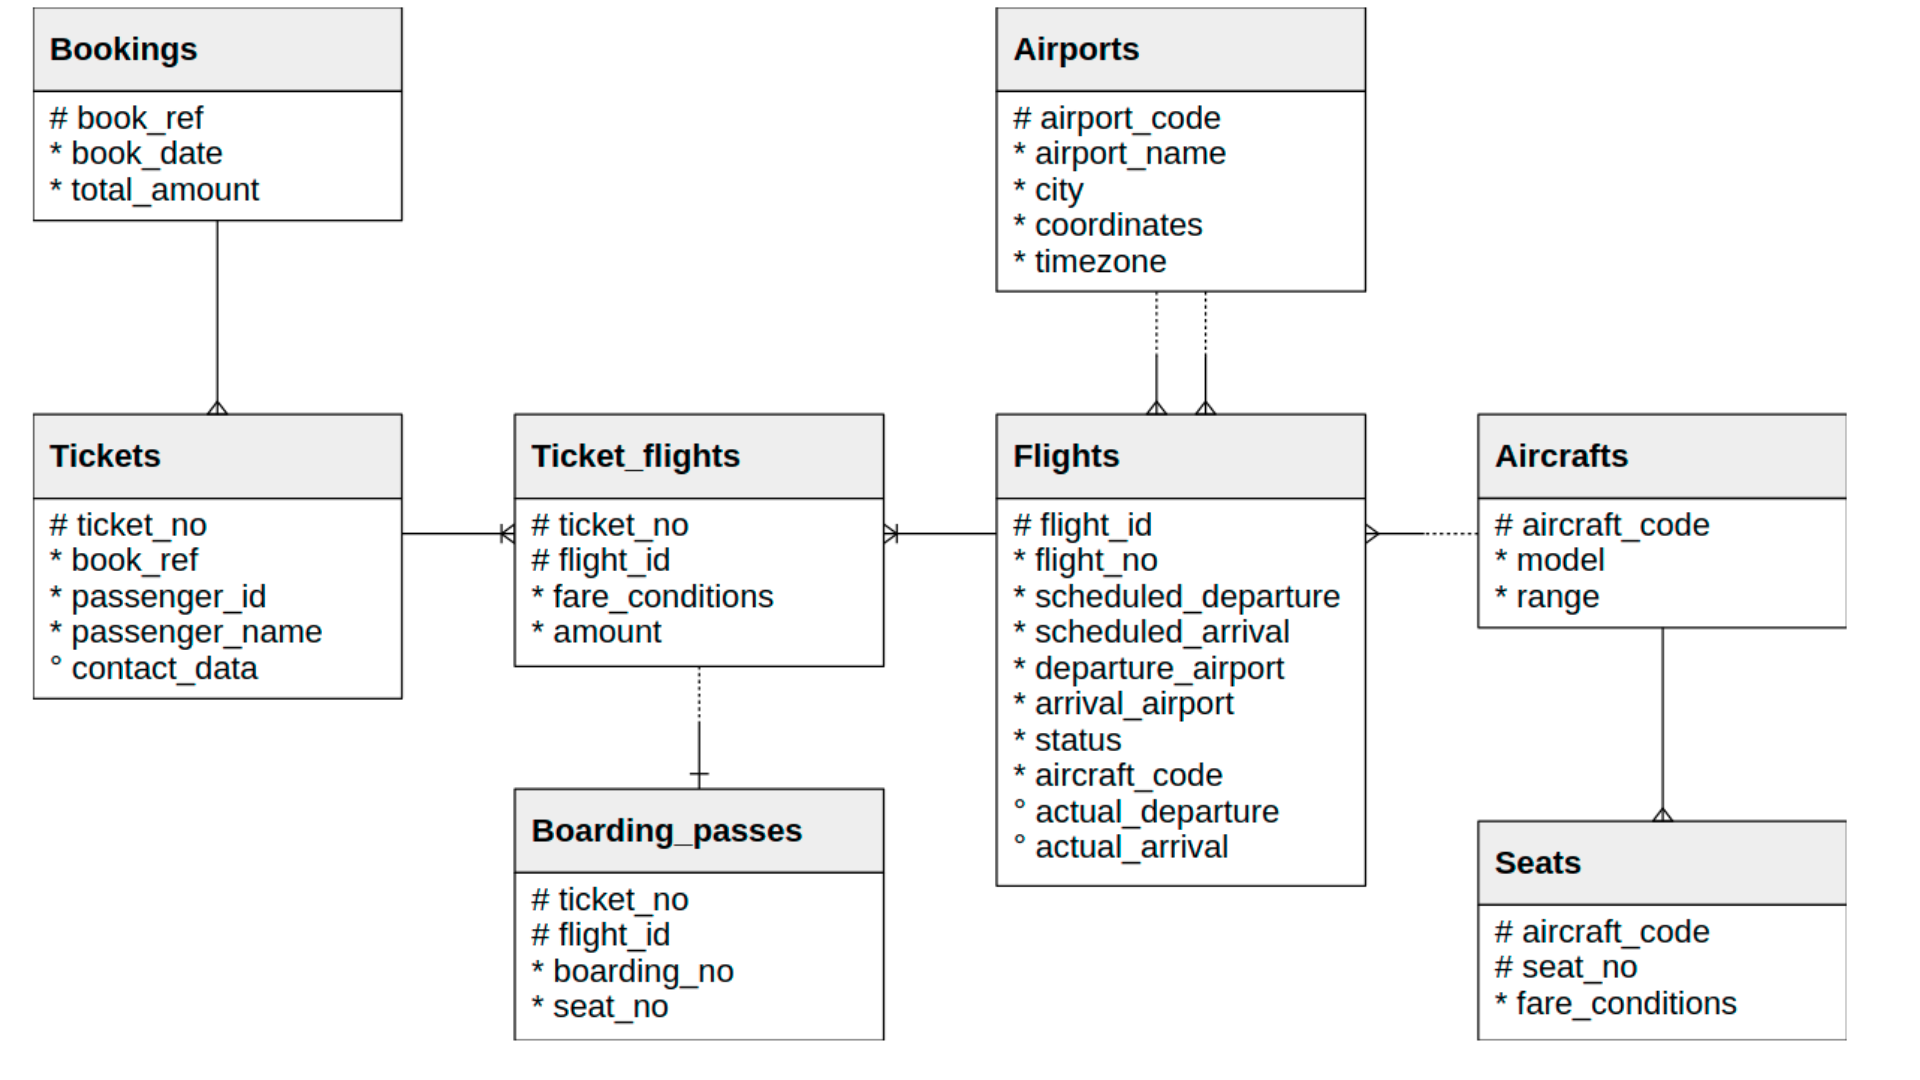
\includegraphics[scale=0.25]{Static/MLD.png} 
    \end{center}
\end{figure}
Les dimensions retenues pour l'\'evaluation de la qualit\'e des donn\'ees sont les suivantes: la compl\'etude, la validit\'e, la coh\'erence, l'exactitude et l'unicit\'e. Les paragraphes suivants pr\'esentent les tokens, les dimensions concern\'ees ainsi que le proc\'ed\'e d'\'evaluation.
\\

La d\'etection des valeurs nulles rel\`eve de la compl\'etude (Token 1). En effet, Griffin au moyen de la dimension \textbf{Completeness} renvoie la r\'epartition valeurs nulles, valeurs compl\`etes et effectif total.  La d\'etection des valeurs aberrantes (Token 2), concourt \`a l'identification des valeurs qui ne sont pas conformes aux d\'efinitions des colonnes en termes de valeurs attendues ou licites. Pour faire le test, nous avons v\'erifi\'e l'existence de valeurs n\'egatives pour la variable '\textit{total\_amounts}'  de la table 'Bookings'. On s'intéresse ainsi \`a l'aspect \textbf{Validit\'e} de la donn\'ees. Il en est de m\^eme lorsqu'on souhaite identifier la plage des valeurs pour les colonnes num\'eriques, les modalit\'es de chaque colonne qualitative ou m\^eme quelques statistiques descriptives (Tokens 3, 4 et 6). La d\'etection des caract\`eres sp\'eciaux dans les cha\^ines de caract\`eres (Token 12) ainsi que la d\'efinition d'expressions r\'eguli\`eres  pour valider le formatage de certaines colonnes (Token 5) sont \'egalement des t\^aches entrant dans la v\'erification de la validit\'e des donn\'ees. Pour la validation de ces diff\'erents \textit{token}, nous avons eu recours cette fois \`a la dimension Profiling de Griffin. En fonction de la complexit\'e du r\'esultat souhait\'e un usage alternatif de \emph{griffin-dsl} et de \emph{spark-sql} a \'et\'e fait.
\\

La dimension de \textbf{Coh\'erence} est couverte par les Tokens 8 et 9. De façon opérationnelle on a : v\'erifi\'e que les valeurs de '\textit{ticket\_no}' dans la table 'Ticket\_flights' existent au niveau de la table 'Ticket' (Token 8)  et impl\'ement\'e des règles de qualit\'e telles que la somme des prix des tickets de chaque vol pour une r\'eservation donn\'ee soit \'egale au total de la r\'eservation (Token 9 ). Afin d'\'evaluer cette dimension, nous avons fait usage de la dimension Profiling de Griffin. Le comptage des doublons (Token 7), fut \'egalement fait au moyen de la dimension Profiling avec du \emph{spark-sql}. Elle fait ressortir le nombre total d’observations dans la colonne, le nombre d’observations distinctes et le nombre d’observations distinctes apparaissant plus d’une fois. Enfin la dimension d'\textbf{Exactitude} est mat\'erialis\'ee ici par l'\'evaluation de l'exactitude entre deux (2) tables. Naturellement, l'usage de la dimension Accuracy de Griffin s'est fait pour valider le Token 11.
%\newpage
\vspace{0.5cm} 
\begin{lstlisting}[language=json,firstnumber=1,caption={Exemple fichier .json : Profiling Seats},captionpos=b]
{ "name": "batch_prof",
  "process.type": "batch",
  "data.sources": [
    { "name": "src",
      "baseline": true,
       "connector": {
                     "type": "jdbc",
                     "config": { "database": "demo",
                     "tablename": "bookings.seats",
                     "url":"jdbc:postgresql://172.18.0.5:5432/demo",
                     "user":"aurel",
                     "password":"123456789",
                     "driver":"org.postgresql.Driver" }
                    }
    }   
  ],
  "evaluate.rule": {
    "rules": [
    {   "dsl.type": "griffin-dsl",
        "dq.type": "profiling",
        "out.dataframe.name": "prof",
        "rule": "src.aircraft_code.count() AS aircraft_code_count",
        "out": [
          { "type": "metric",
            "name": "prof"   }
        ]
     }
   ]
  },
  "sinks": ["CONSOLE", "HDFS", "ELASTICSEARCH"] }
\end{lstlisting}
\vspace{0.15cm}

Suite \`a la validation des tokens, une base de donn\'ees fictives sur l'assurance automobile nous a \'et\'e confi\'ee, pour l'\'evaluation de la qualit\'e. Cette \'evaluation s'est faite sans instructions particuli\`eres. Les donn\'ees sur l'assurance automobile n'\'etaient constituées que d'une seule table. On y trouve : le num\'ero de police, les dates de d\'ebut et de fin de police, la fr\'equence de paiement (annuelle ou mensuelle), la langue du contrat, la profession, le type de territoire (urbain, rural ou semi-urbain), l'utilisation faite du v\'ehicule,  la pr\'esence d'alarme, la marque du v\'ehicule, le genre du conducteur, son \^age, la dur\'ee de son permis de conduire, l'ann\'ee de mise en circulation du v\'ehicule, le nombre de sinistre, l'exposition aux sinistres ainsi que les divers co\^uts li\'es aux garanties et au contrat d'assurance. Sur cette table, les dimensions de complétude, de validité, de cohérence, et d’unicité ont \'et\'e \'evalu\'e cette fois. Afin d'idenifier les r\`egles de coh\'erence nous avons \'emis certaines hypoth\`eses. Nous avons produit les m\'etriques suivantes, telles que repr\'esent\'ees sur Kibana: 
%\newpage    
\begin{figure}[!htp]
    \caption{Aperçu des m\'etriques calcul\'ees }  \label{fig:edge34}
  \begin{center}
    \subfigure[Compl\'etude]{\label{fig:edge-34a}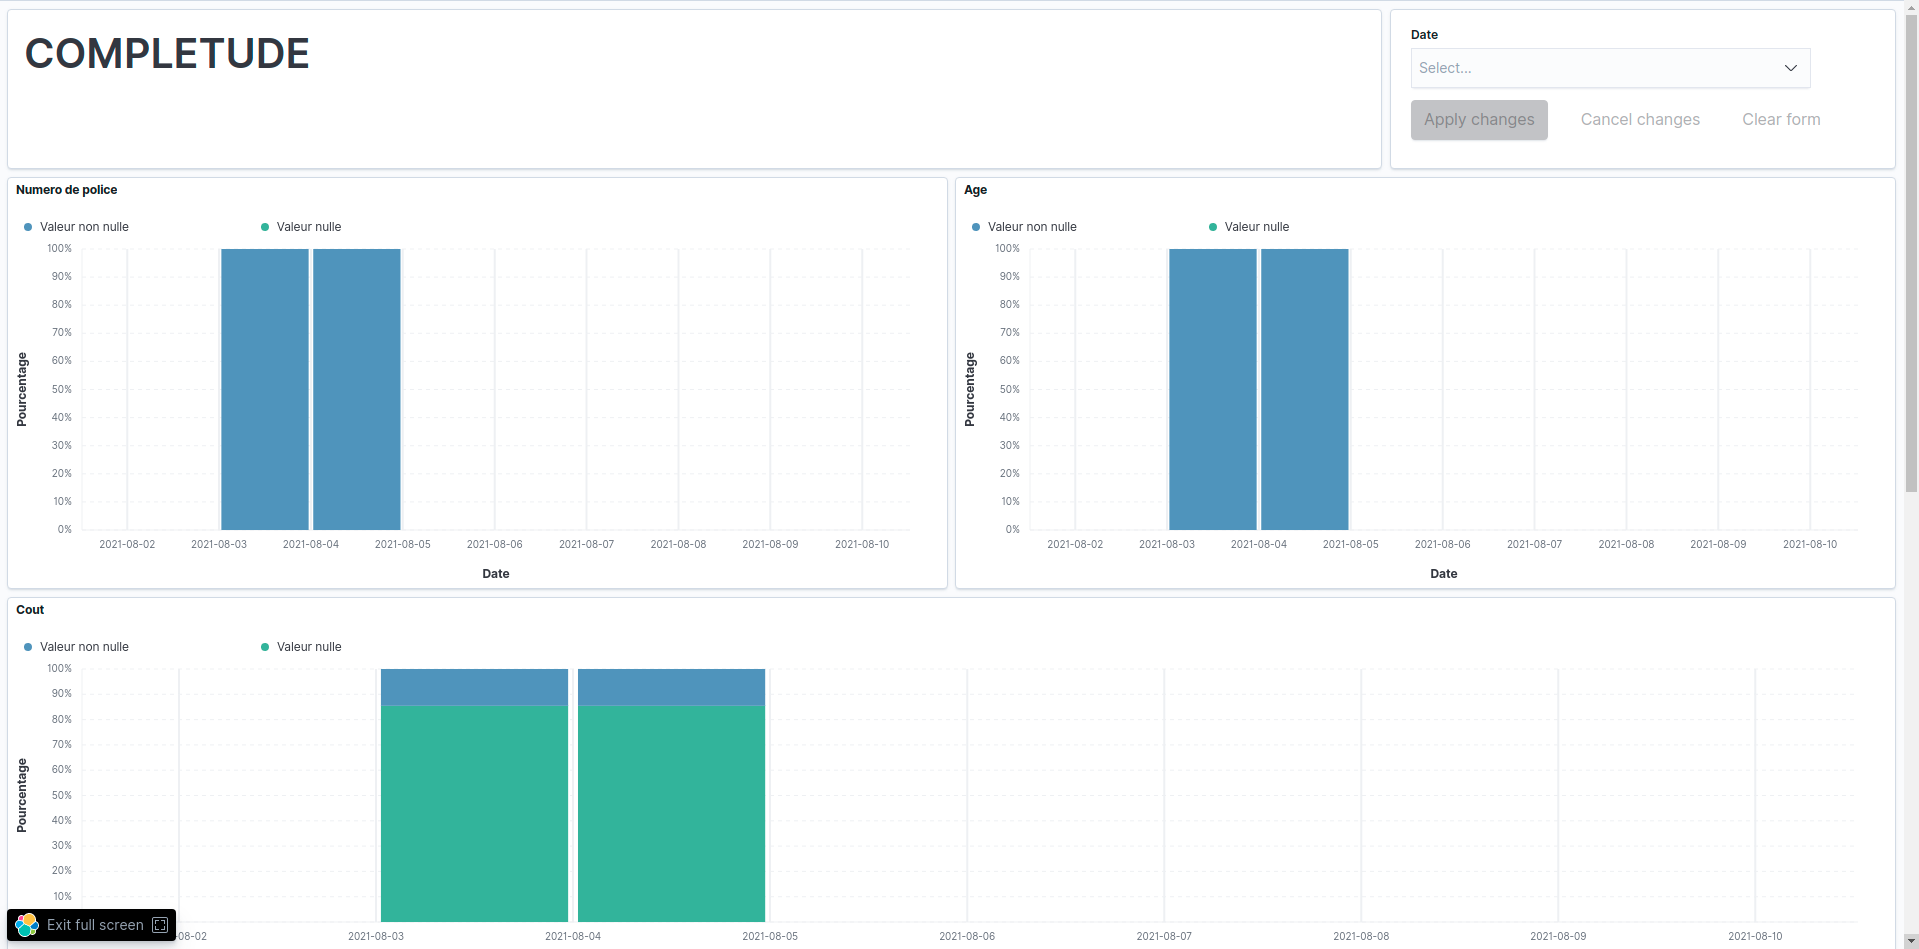
\includegraphics[scale=0.12]{Static/Captures_d_ecran_dashboard/Completetude.png}}
    \subfigure[Unicit\'e]{\label{fig:edge-34b}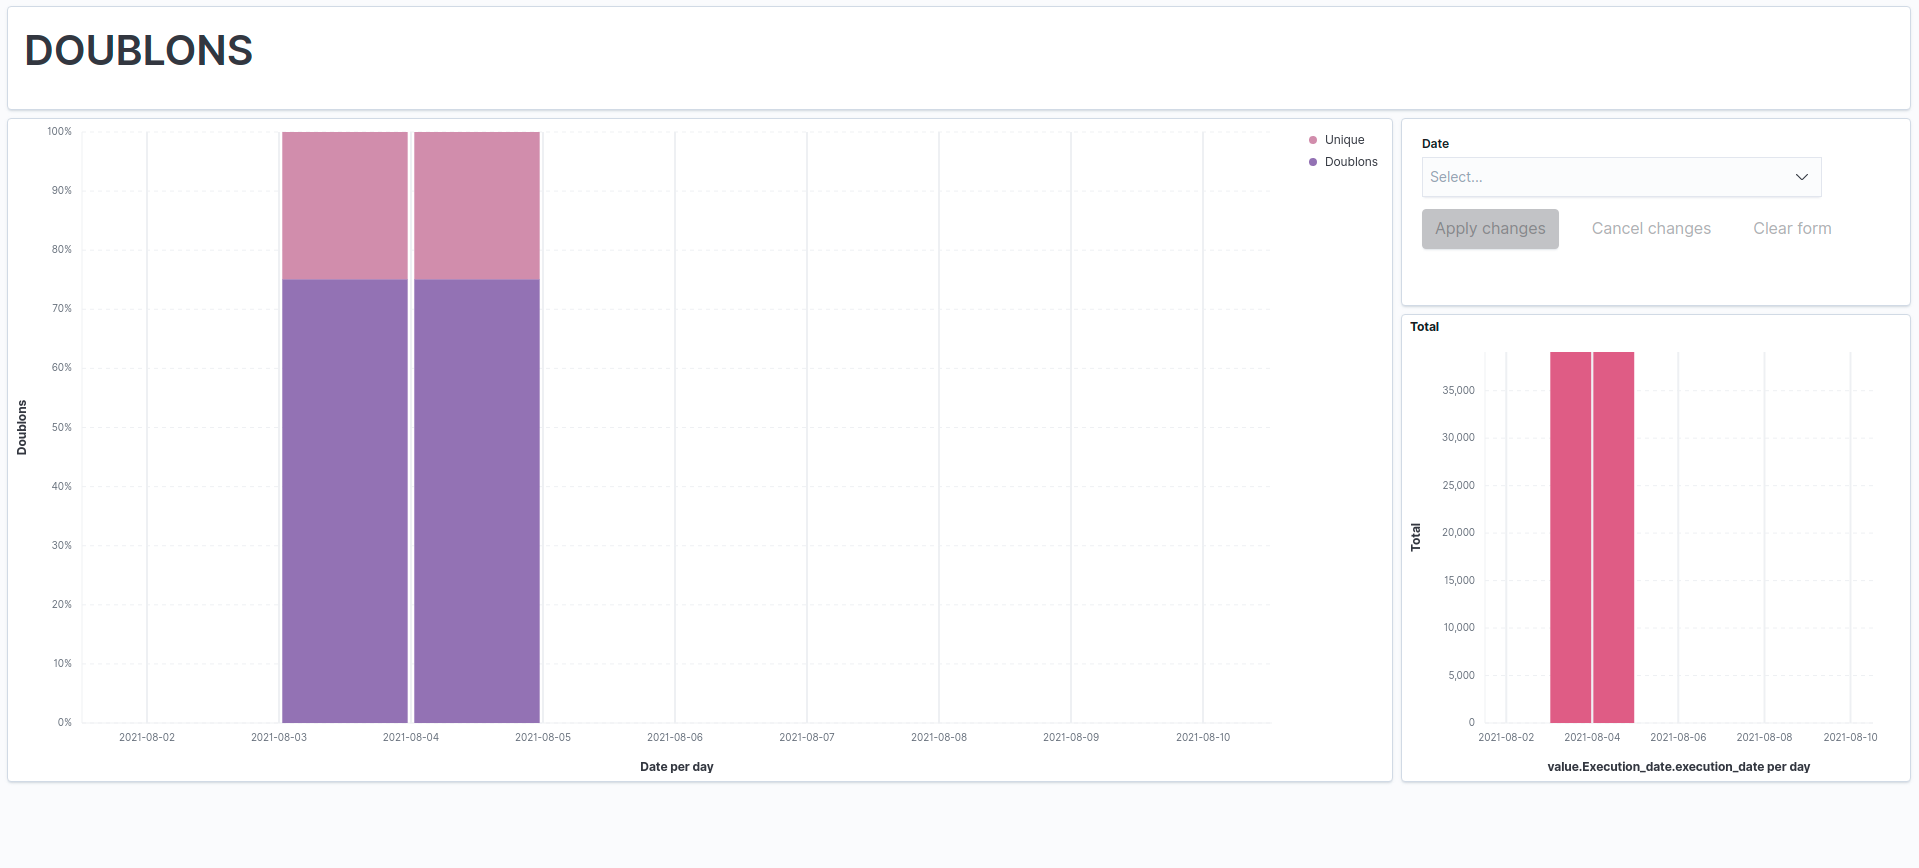
\includegraphics[scale=0.12]{Static/Captures_d_ecran_dashboard/Doublons.png}} 
  
    \subfigure[Incoh\'erence]{\label{fig:edge-34c}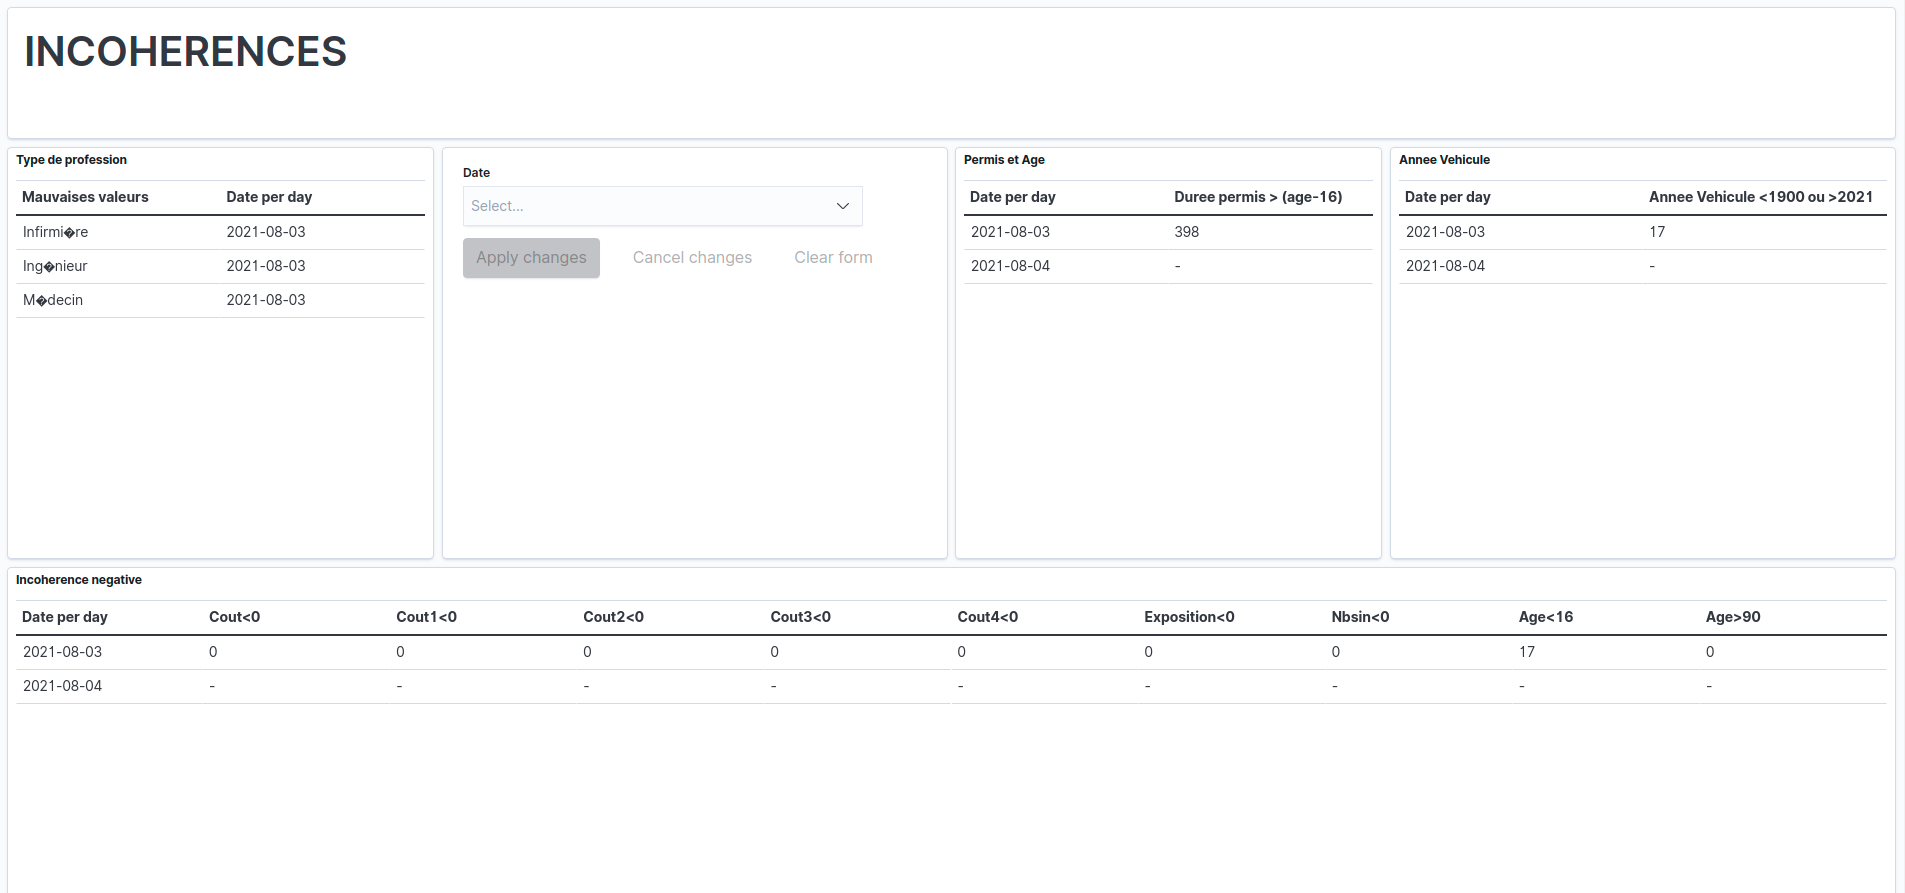
\includegraphics[scale=0.12]{Static/Captures_d_ecran_dashboard/Incoherences1.png}}
  	\subfigure[Validit\'e]{\label{fig:edge-34d}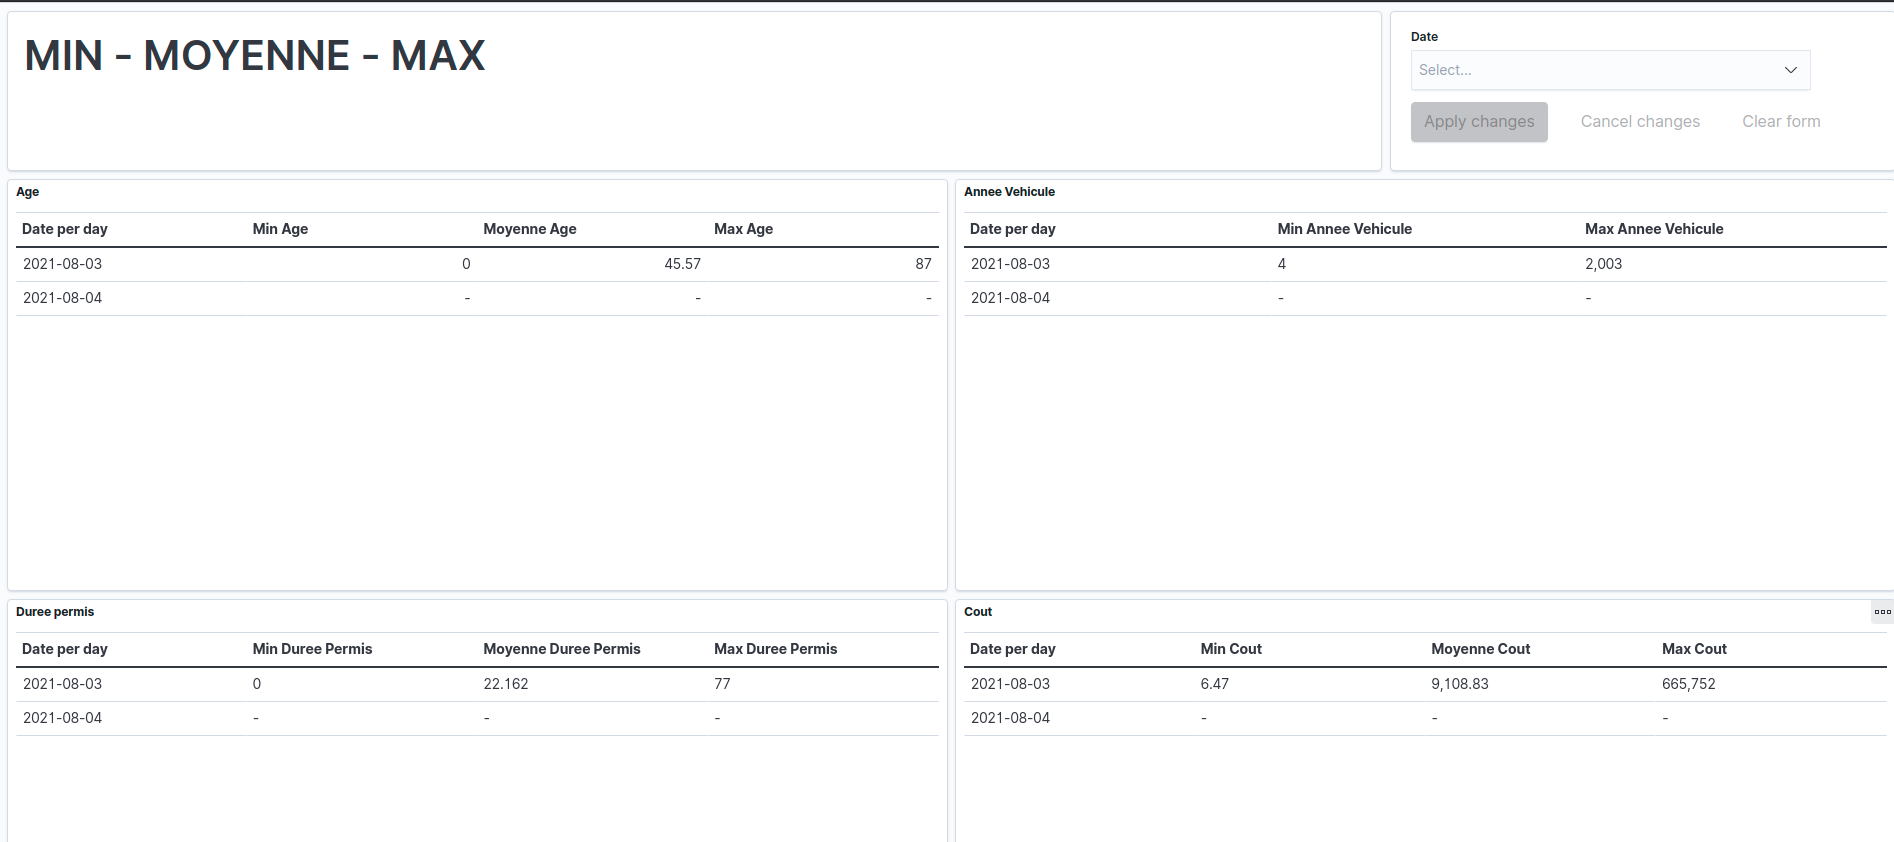
\includegraphics[scale=0.12]{Static/Captures_d_ecran_dashboard/Stats_Desc.png}}
  \end{center}
\end{figure}
